\section{Theorie}
In diesem Versuch werden Relaxationsvorgänge betrachtet. Bei einer Relaxation kehrt
ein zuvor gestörtes System nicht-oszillatorisch in seinen Gleichgewichtszustand
zurück. Das System verfügt über eine charakteristische Größe $A$. Ist es linear,
so folgt die Änderungsgeschwindigkeit zum Zeitpunkt $t$ der Gleichung
\begin{equation}
  \frac{\symup{d}A}{\symup{d}t}(t) = c[A(t)-A(t \to \infty)]\,.
  \label{eqn:linearrelax}
\end{equation}
Dabei ist A(t \to \infty) der nur asymptotisch erreichbare Wert der Größe $A$ im
Gleichgewichtszustand, $c$ ist eine Konstante größer Null, sodass A beschränkt
bleibt.
Wird \eqref{eqn:linearrelax} nach der Zeit integriert, ergibt sich für $A$ die
exponentielle Zuordnung
\begin{equation}
  A(t) = A(t \to \infty) + [A(0) - A(t \to \infty)] \exp(ct)\,.
\end{equation}
Die in diesem Versuch untersuchten Relaxationsvorgänge sind der Auf- und Entladevorgang
eines Kondensators über einen Widerstand. Der Schaltplan hierzu ist in \ref{fig:Aufbau_1} zu sehen.
\begin{figure}
  \centering
  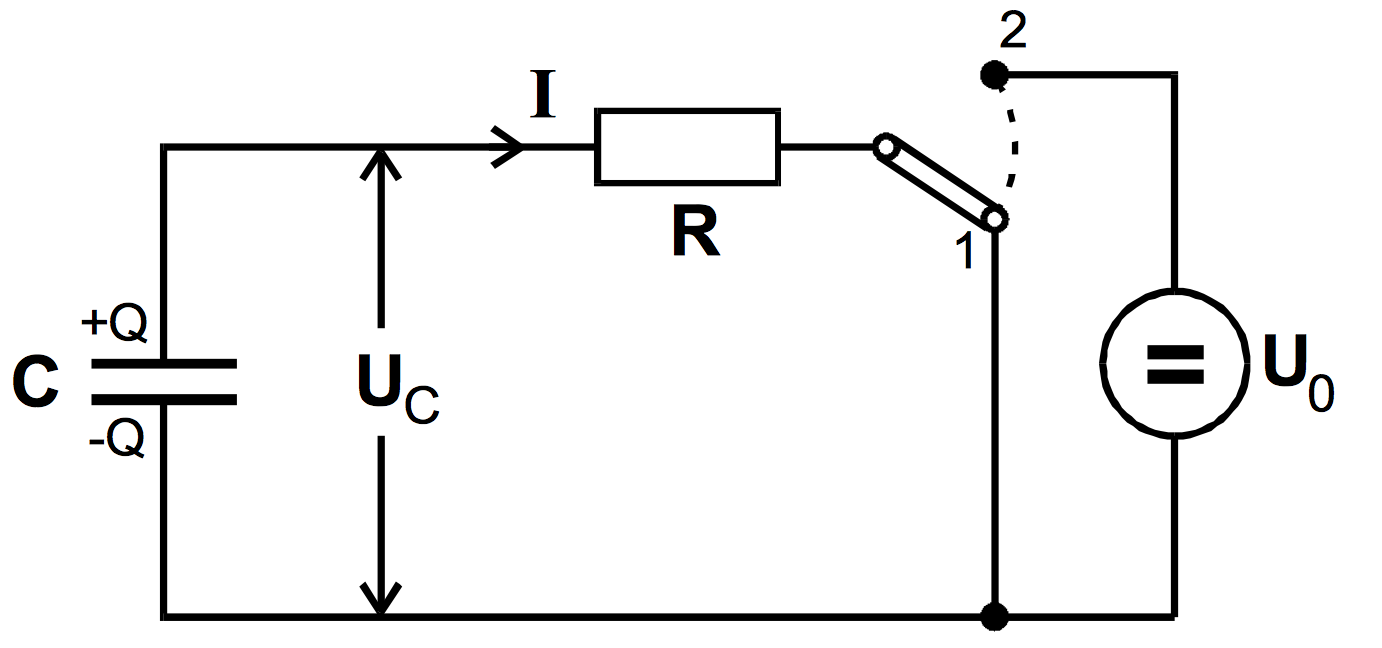
\includegraphics[width=260pt]{aufbau_1.png}
  \caption{Beispielhafte Schaltung zur Auf- und Entladung eines Kondensators über einen
  Widerstand unter Verwendung von Gleichspannung \cite{Versuchsanleitung}}
  \label{fig:Aufbau_1}
\end{figure}


Stets liegt auf den Kondensatorplatten zum Zeitpunkt $t$ eine Ladung $Q(t)$. Für
die am Kondensator anliegende Spannung $U_{\text{C}}$ gilt dann
\begin{equation}
  U_{\text{C}} = Q / C\,,
\end{equation}
wobei $C$ die Kapazität des Kondensators ist. Da der Kondensator mit dem Widerstand
in Reihe geschaltet ist, bewirkt die am Kondensator abfallende Spannung $U_{\text{C}}$
gemäß dem Ohmschen Gesetz den Strom
\begin{equation}
  I = U_{\text{C}} / R\,.
\end{equation}
Zusammen mit der Beziehung $\dot{Q} = -I$ lässt sich eine zu \eqref{eqn:linearrelax}
analoge Differentialgleichung für $Q(t)$ mit der asymptotischen Randbedingung
$Q(t \to \infty) = 0$, da es sich um einen Entladevorgang handelt, aufstellen. Die
Lösung dieser ist
\begin{equation}
  Q(t) = Q(0) \exp(-t/\tau)
  \label{eqn:kondensatorqrelax}
\end{equation}
mit der Zeitkonstanten $\tau \coloneqq RC$ des RC-Glieds.
Da bei einem Kondensator die Spannung $U_\text{C}(t)$ proportional zur Ladung
$Q(t)$ auf den Kondensatorplatten ist, wird analog zu \eqref{eqn:kondensatorqrelax}
die Kondensatorspannung der Zuordnung
\begin{equation}
  U_\text{C}(t) = U_\text{C}(0) \exp(-t/\tau)
  \label{eqn:kondensatorurelax}
\end{equation}
folgen.


Wird an den das RC-Glied eine Spannung $U_{\text{G}}=U_{\text{0}}cos(\omega t)$ angelegt, deren
Frequenz klein gegen $\frac{1}{RC}$ ist, so folgt der Spannungsverlauf am Kondensator
dem der Quelle. Wird die Frequenz jedoch erhöht, so stellt sich eine Phasenverschiebung
zwischen Generatorspannung $U_{\text{G}}$ und der Spannung $U_{\text{C}}$ am Kondensator
ein, bei der die Generatorspannung der Spannung am Kondensator vorausläuft.
Zudem nimmt die Amplitude der Spannung am Kondensator ab, da der Kondensator in einer
Periodendauer nicht mehr vollständig geladen werden kann. Ein Schaltplan hierzu findet
sich in \ref{fig:Aufbau_2}.
\begin{figure}
  \centering
  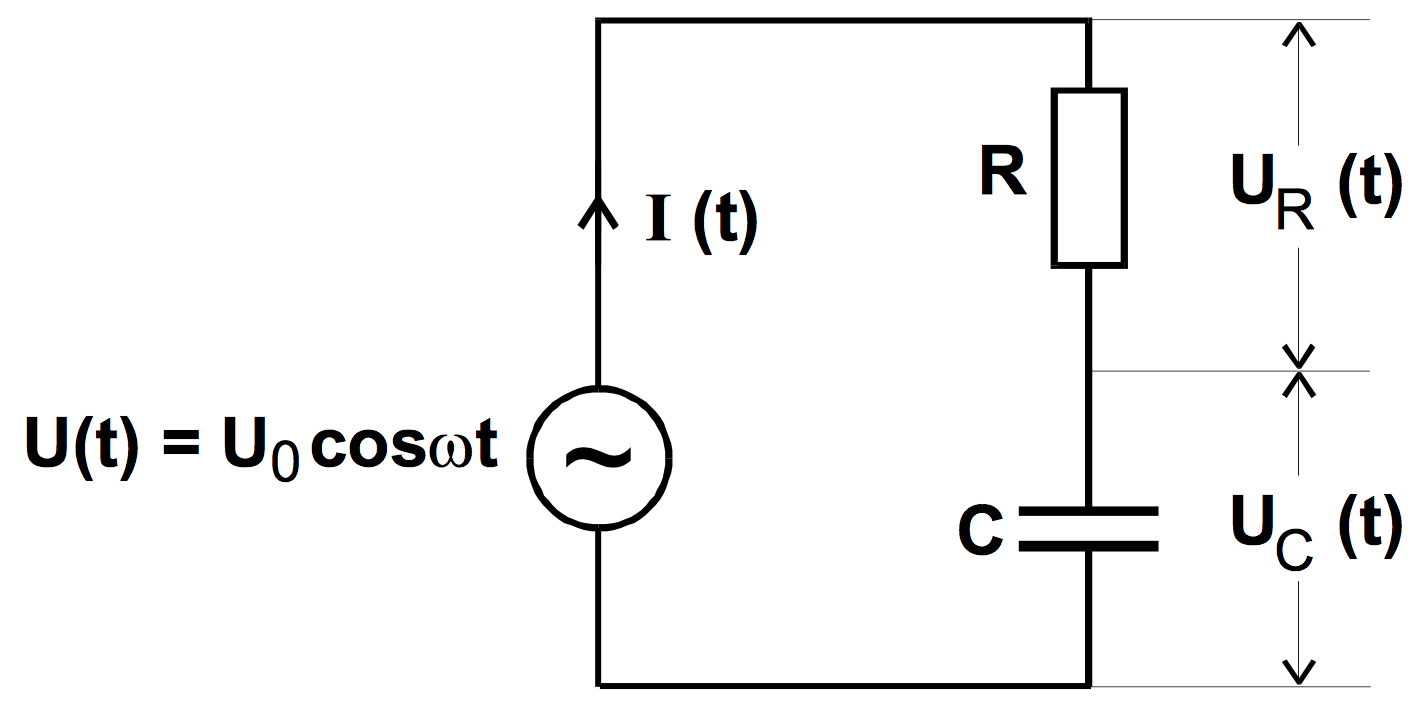
\includegraphics[width=250pt]{aufbau_2.png}
  \caption{Beispielhafte Schaltung zur Auf- und Entladung eines Kondensators über
  einen Widerstand unter Verwendung von Wechselspannung \cite{Versuchsanleitung}}
  \label{fig:Aufbau_2}
\end{figure}


Um eine Lösung für die Phasenverschiebung zu erhalten, wird der Ansatz
\begin{equation}
  U_{\text{C}}(t)=A(\omega)cos(\omega t + \phi(\omega))
\end{equation}
gewählt. Dieser lässt sich mithilfe der Kirchhoff'schen Regeln und der Beziehung
\begin{equation}
  I(t)=\frac{dQ}{dt}=C\frac{dU_{\text{C}}}{dt}
\end{equation}
zur Formel für die Frequenzabhängigkeit der Phase $\phi$ umformen. Es ergibt sich die
Beziehung
\begin{equation}
  \phi(\omega)=arctan(-\omega R C) \,.
\end{equation}
Der Wert der Phasenverschiebung geht also für kleine Frequenzen gegen $0$ und für
große Frequenzen gegen $\frac{\pi}{2}$. Für $\omega=\frac{1}{RC}$ nimmt sie den Wert
$\frac{\pi}{4}$ an.
Durch einige weitere Überlegungen lässt ergibt sich hieraus
\begin{equation}
  A(\omega)=\frac{U_{\text{0}}}{\sqrt{1+\omega^2 R^2 C^2}} \,,
\end{equation}
wobei $U_{\text{0}}$ die Amplitude der Generatorspannung $U_{\text{G}}$ und $A$ die
Amplitude der Spannung $U_{\text{C}}$ am Kondensator ist.
Man kann erkennen, dass die Amplitude am Kondensator für kleine $\omega$ gegen $U_{\text{0}}$ geht
und mit steigendem $\omega$ sinkt. Für $\omega=\frac{1}{RC}$ nimmt sie den Wert
$\frac{U_{\text{0}}}{\sqrt{2}}$ an.

Werden an das RC-Glied Wechselspannungen mit sehr hoher Frequenz angelegt, so kann
am Kondensator eine zu $\int U(t)\,\symup{d}t$ proportionale Spannung beobachtet werden.
Bei hohen Frequenzen gilt $\lvert U_{\text{C}} \rvert << \lvert U_{\text{R}} \rvert$
und $\lvert U_{\text{C}} \rvert << \lvert U \rvert$. Somit ergibt sich näherungsweise
aus den Kirchhoff'schen Gesetzen mit einigen Umformungen
\begin{gather}
  U(t)= R C \frac{\symup{d}U_{\text{C}}}{\symup{d}t} \\
  U_{\text{C}}(t)=\frac{1}{RC}\int_0^t U(t')\, dt'
\end{gather}



\label{sec:Theorie}
